\chapter{Environment Driven Taxa Clusters}

%% ============================================
%% RDA Analysis Tables
%% ============================================

\begin{table}[htbp]
    \centering
    \caption{RDA Axes Summary}
    \label{tab:03_rda_axes}
    \small
    \begin{tabular}{lccccc}
        \toprule
        \textbf{Axis} & \textbf{Eigenvalue} & \textbf{Expl. (\%)} & \textbf{Cumul. (\%)} & \textbf{F-stat} & \textbf{p-value} \\
        \midrule
        RDA1 & 0.0295 & 44.53 & 44.53 & 5.789 & 0.001$^{**}$ \\
        RDA2 & 0.0155 & 23.42 & 67.95 & 3.044 & 0.151 \\
        RDA3 & 0.0119 & 17.98 & 85.93 & 2.338 & 0.483 \\
        RDA4 & 0.0047 & 7.15 & 93.08 & 0.929 & 1.000 \\
        RDA5 & 0.0026 & 3.98 & 97.06 & 0.517 & 1.000 \\
        RDA6 & 0.0020 & 2.94 & 100.00 & 0.383 & 1.000 \\
        \bottomrule
    \end{tabular}
    
    \vspace{0.5em}
    \footnotesize
    \textit{Note:} Permutations = 999; $R^2$ = 0.2167; Adjusted $R^2$ = 0.1167; Global test p-value = 0.0010$^{**}$
\end{table}

\begin{table}[htbp]
    \centering
    \caption{RDA Environmental Terms}
    \label{tab:03_rda_env_terms}
    \small
    \begin{tabular}{l@{\hspace{8pt}}c@{\hspace{8pt}}c@{\hspace{8pt}}c@{\hspace{8pt}}r@{\hspace{8pt}}r}
        \toprule
        \textbf{Variable} & \textbf{$\Delta$ Inertia} & \textbf{F-stat} & \textbf{p-value} & \textbf{RDA1} & \textbf{RDA2} \\
        \midrule
        MPS (Phi) & 1.204 & 4.459 & 0.001$^{**}$ & $-0.900$ & 0.088 \\
        Velocity (m/sec) & 0.624 & 2.310 & 0.016$^{*}$ & 0.361 & 0.165 \\
        Depth (m) & 0.478 & 1.769 & 0.065 & 0.456 & $-0.442$ \\
        Temperature (\textdegree C) & 0.424 & 1.572 & 0.112 & $-0.046$ & 0.699 \\
        DO Bottom (mg/L) & 0.340 & 1.258 & 0.235 & $-0.108$ & $-0.628$ \\
        LOI (\%) & 0.185 & 0.684 & 0.747 & 0.136 & 0.228 \\
        \bottomrule
    \end{tabular}
\end{table}

\begin{figure}[htbp]
    \centering
    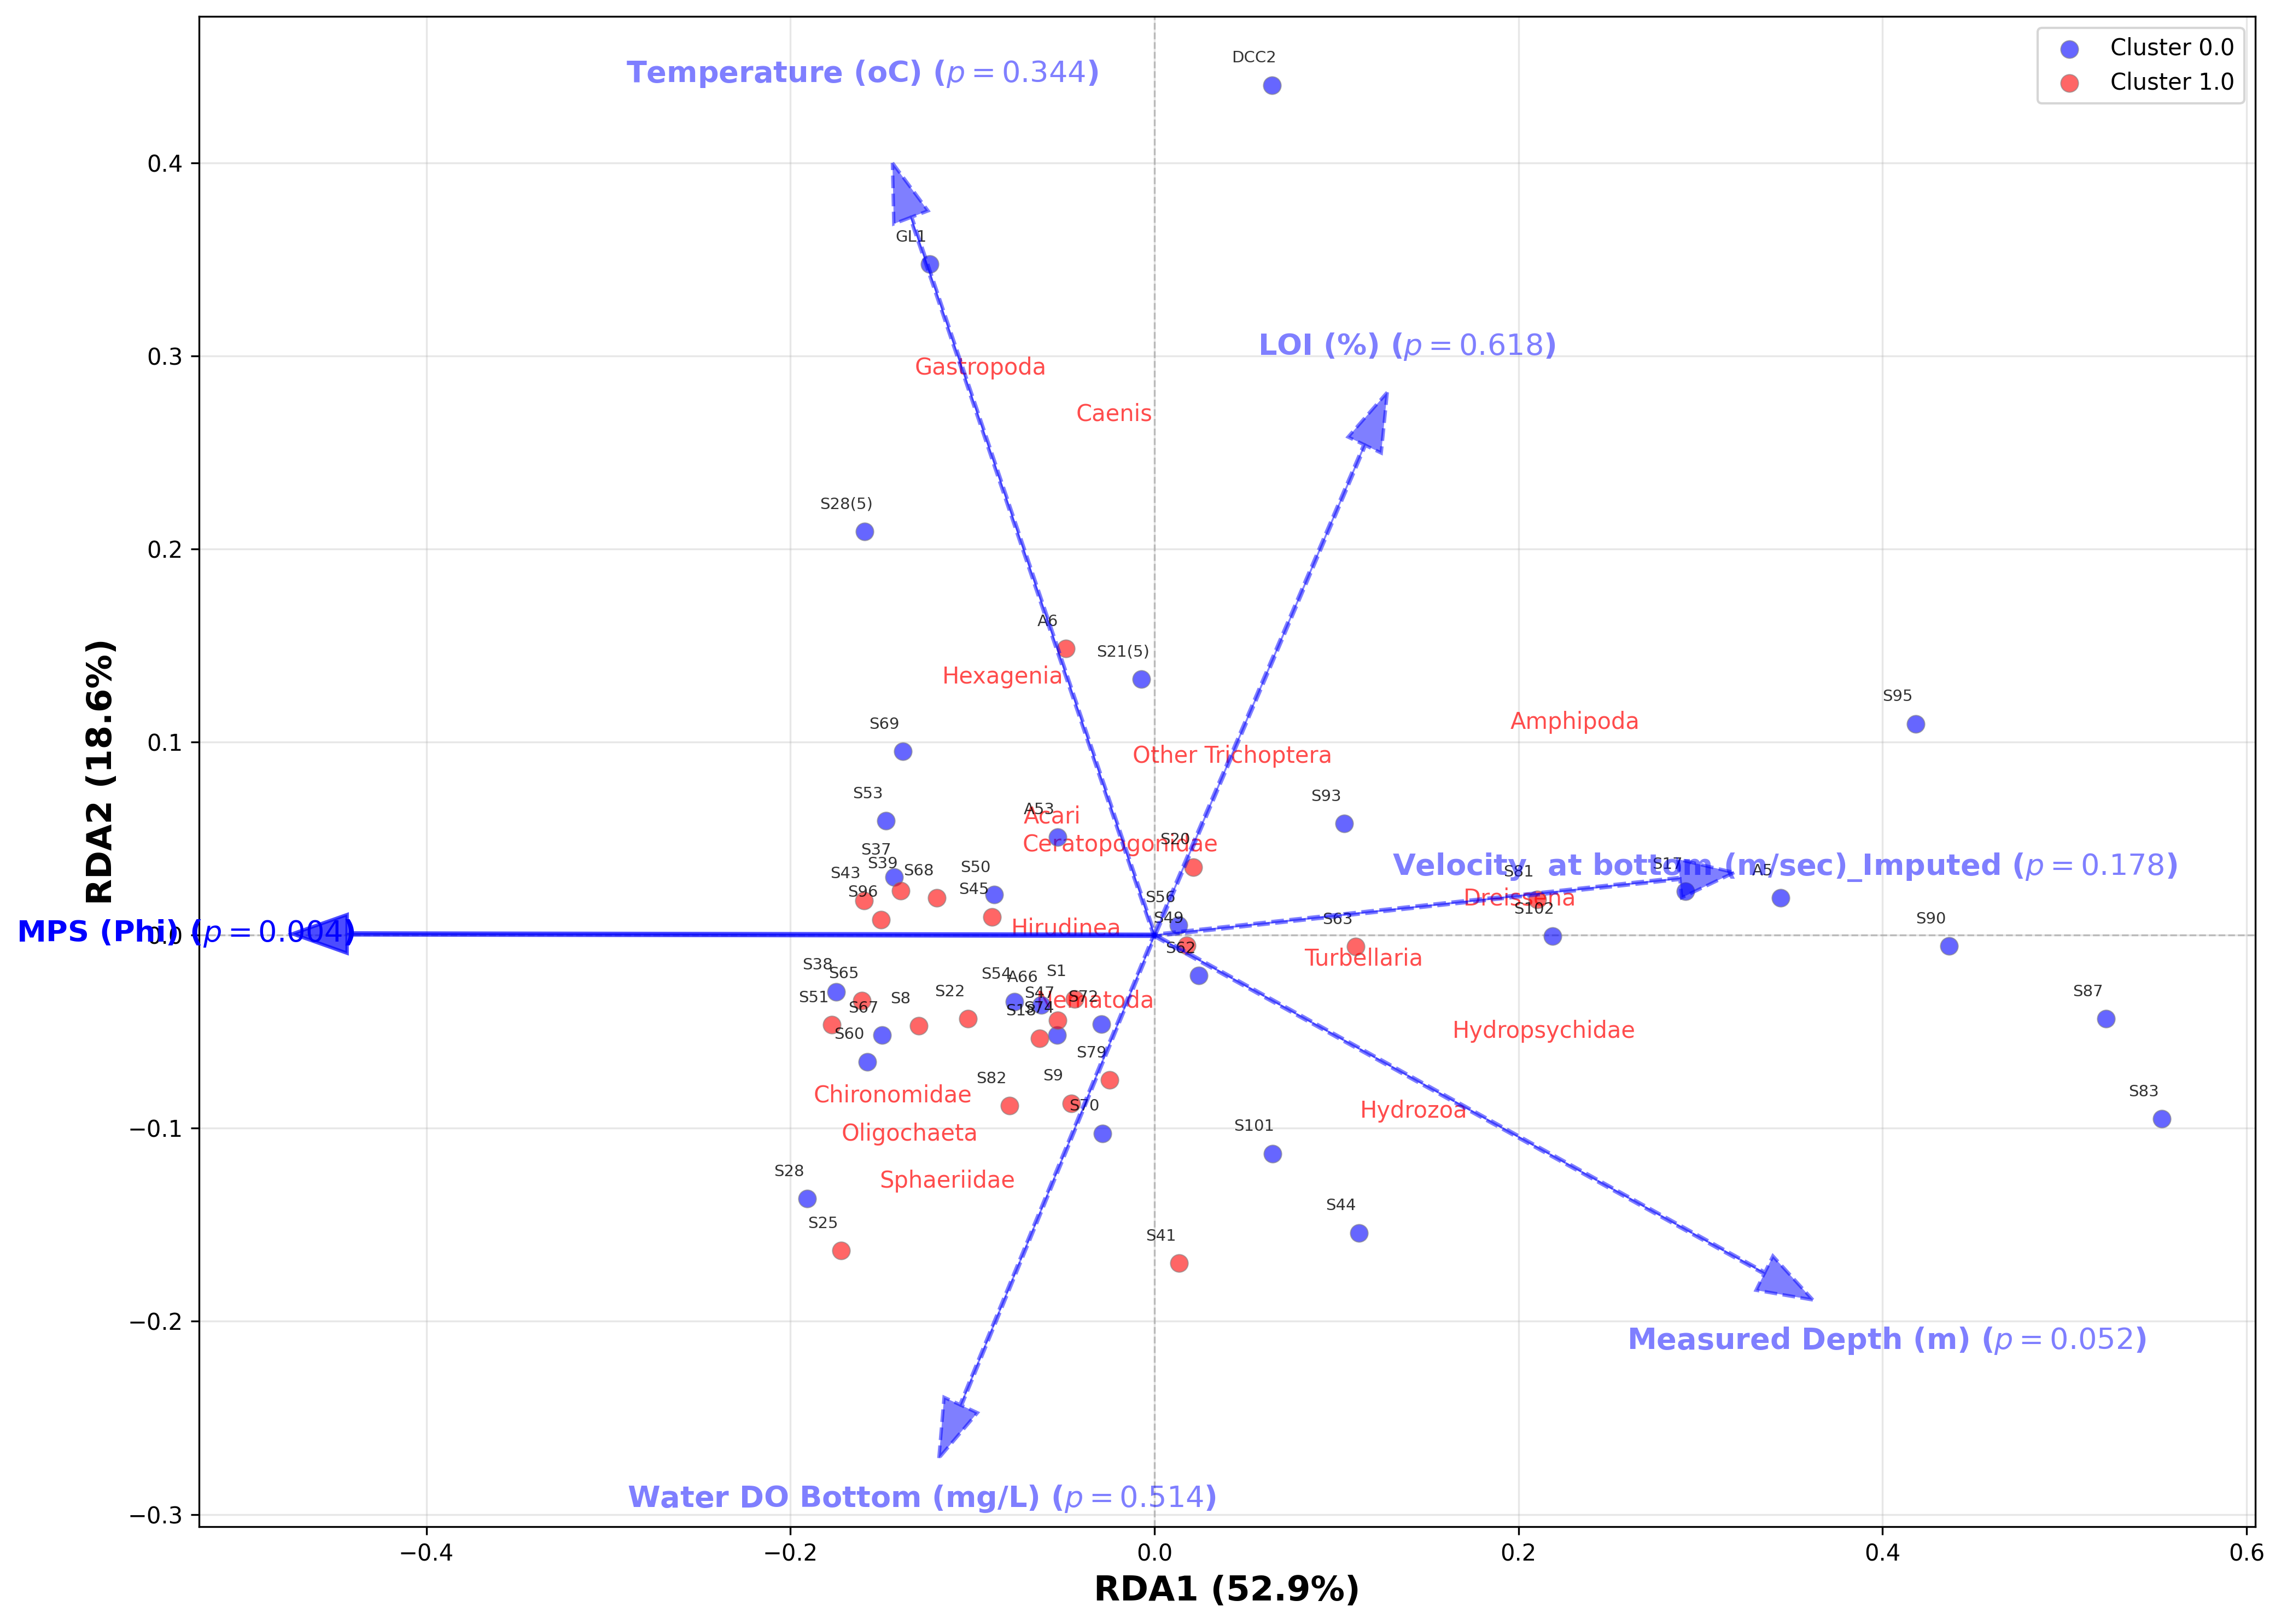
\includegraphics[width=0.9\textwidth]{../results/figures/03_env_driven_taxa_clusters/figure1_rda_triplot.png}
    \caption{RDA Triplot}
    \label{fig:03_rda_triplot}
\end{figure}

% \begin{figure}[htbp]
%     \centering
%     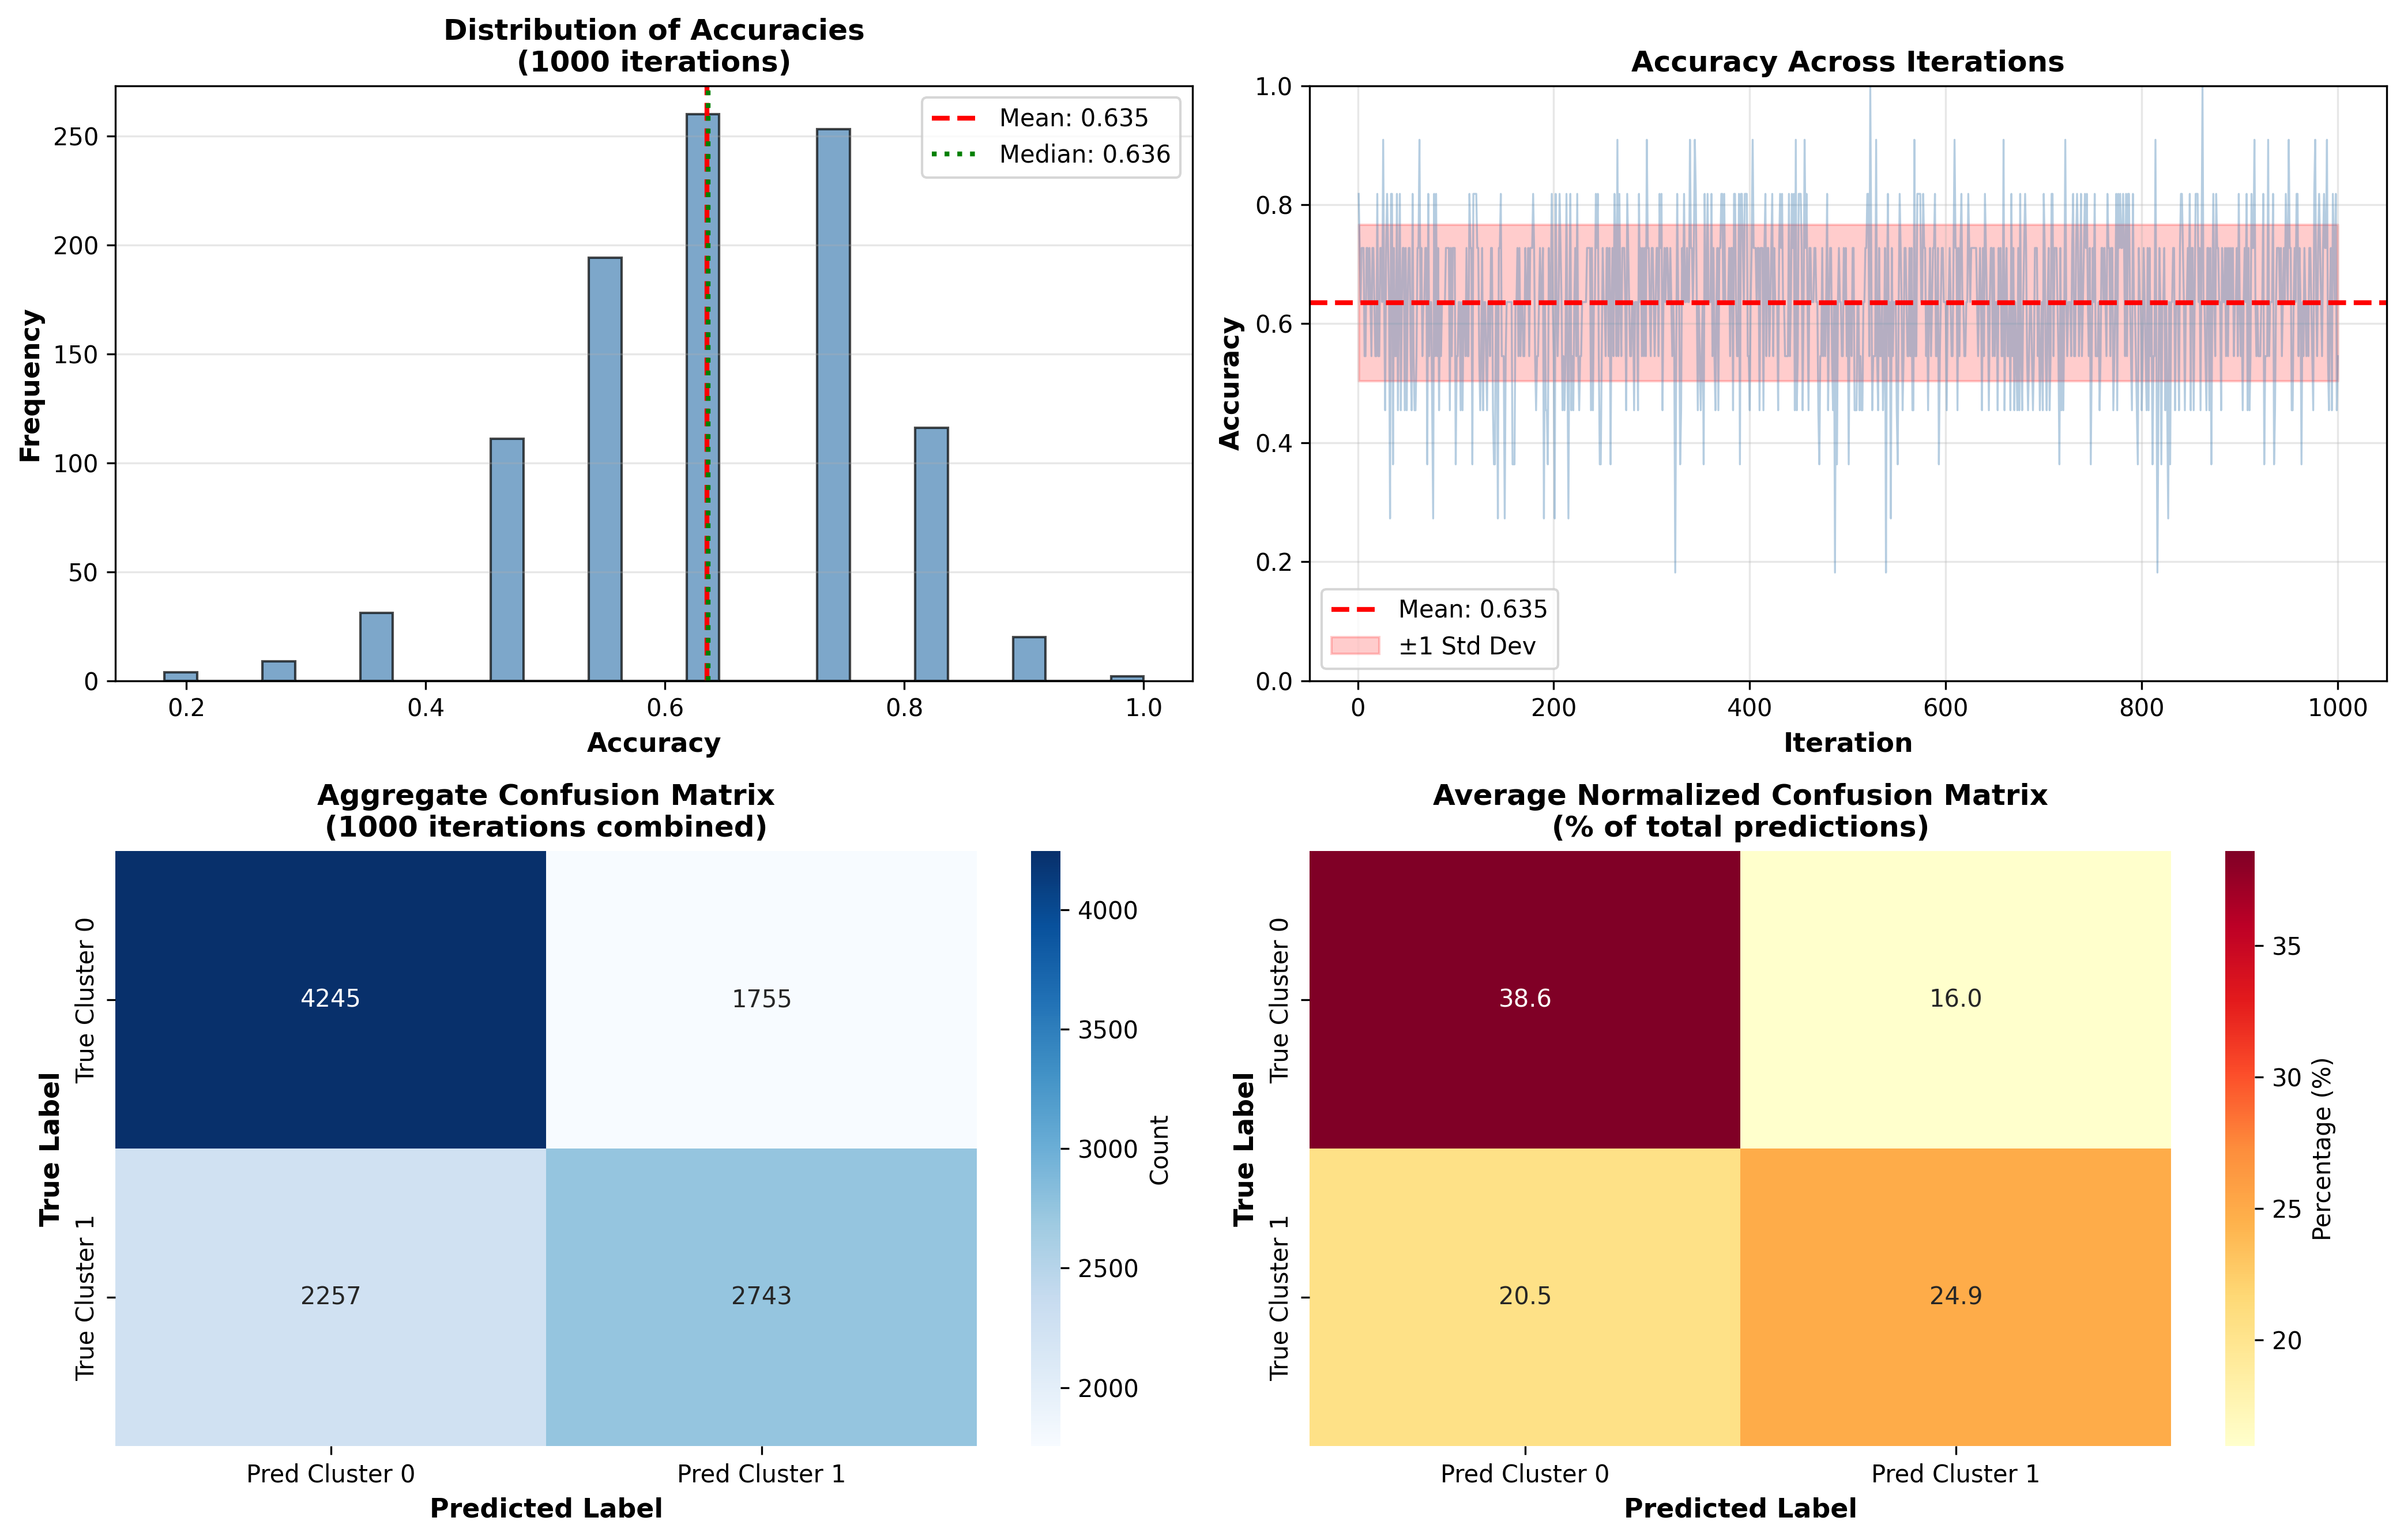
\includegraphics[width=0.9\textwidth]{../results/figures/03_env_driven_taxa_clusters/figure2_lda_cv.png}
%     \caption{LDA Cross-Validation}
%     \label{fig:03_lda_cv}
% \end{figure}

%% ============================================
%% LDA Analysis Tables
%% ============================================

\begin{table}[htbp]
    \centering
    \caption{LDA Variable Importance (Wilks' Lambda) and Discriminant Axes Summary}
    \label{tab:03_lda_analysis}
    \small
    \begin{tabular}{l@{\hspace{8pt}}c@{\hspace{8pt}}c@{\hspace{8pt}}c@{\hspace{8pt}}r@{\hspace{8pt}}r}
        \toprule
        \textbf{Variable} & \textbf{$\Delta\Lambda$} & \textbf{F-stat} & \textbf{p-value} & \textbf{LD1} & \textbf{LD2} \\
        \midrule
        MPS (Phi) & 0.130 & 6.926 & 0.002$^{**}$ & $-0.924$ & 0.666 \\
        Temperature (\textdegree C) & 0.119 & 6.336 & 0.004$^{**}$ & 0.388 & $-0.667$ \\
        Velocity (m/sec) & 0.104 & 5.534 & 0.007$^{**}$ & $-0.781$ & 0.185 \\
        Depth (m) & 0.087 & 4.617 & 0.015$^{*}$ & 0.552 & $-0.010$ \\
        DO Bottom (mg/L) & 0.022 & 1.186 & 0.315 & 0.088 & 0.156 \\
        LOI (\%) & 0.000 & 0.024 & 0.976 & $-0.021$ & $-0.013$ \\
        \midrule
        \textbf{Explained (\%)} & -- & -- & -- & 59.44 & 40.56 \\
        \textbf{Cumulative (\%)} & -- & -- & -- & 59.44 & 100.00 \\
        \bottomrule
    \end{tabular}
\end{table}

%% ============================================
%% LDA Classification Results
%% ============================================

\begin{table}[htbp]
    \centering
    \caption{LDA Classification Confusion Matrix (Training Data)}
    \label{tab:03_lda_confusion}
    \small
    \begin{tabular}{lccc}
        \toprule
        & \textbf{Pred. Cluster 0} & \textbf{Pred. Cluster 1} & \textbf{Pred. Cluster 2} \\
        \midrule
        True Cluster 0 & 12 & 5 & 1 \\
        True Cluster 1 & 3 & 25 & 0 \\
        True Cluster 2 & 1 & 3 & 4 \\
        \bottomrule
    \end{tabular}
\end{table}

\begin{table}[htbp]
    \centering
    \caption{LDA Classification Report (Training Data)}
    \label{tab:03_lda_classification}
    \small
    \begin{tabular}{lcccc}
        \toprule
        & \textbf{Precision} & \textbf{Recall} & \textbf{F1-Score} & \textbf{Support} \\
        \midrule
        Cluster 0 & 0.75 & 0.67 & 0.71 & 18 \\
        Cluster 1 & 0.76 & 0.89 & 0.82 & 28 \\
        Cluster 2 & 0.80 & 0.50 & 0.62 & 8 \\
        \midrule
        Accuracy & -- & -- & 0.76 & 54 \\
        Macro avg & 0.77 & 0.69 & 0.71 & 54 \\
        Weighted avg & 0.76 & 0.76 & 0.75 & 54 \\
        \bottomrule
    \end{tabular}
    
    \vspace{0.5em}
    \footnotesize
    \textit{Note:} Overall Accuracy = 0.7593; Number of sites = 54
\end{table}

%% ============================================
%% LDA Monte Carlo Cross-Validation Results
%% ============================================
\begin{table}[htbp]
    \centering
    \caption{LDA Monte Carlo Cross-Validation Aggregate Confusion Matrix (Test Size: 20.0\% per 1000 iteration)}
    \label{tab:03_lda_cv_confusion_aggregate}
    \small
    \begin{tabular}{lccc}
        \toprule
        & \textbf{Pred. Cluster 0} & \textbf{Pred. Cluster 1} & \textbf{Pred. Cluster 2} \\
        \midrule
        True Cluster 0 & 2178 & 1486 & 336 \\
        True Cluster 1 & 944 & 4901 & 155 \\
        True Cluster 2 & 237 & 389 & 374 \\
        \bottomrule
    \end{tabular}
    
    \vspace{0.5em}
    \footnotesize
    \textit{Note:} Combined results from 1,000 cross-validation iterations
\end{table}

\begin{table}[htbp]
    \centering
    \caption{LDA Monte Carlo Cross-Validation Results Summary (Test Size: 20.0\% per 1000 iteration)}
    \label{tab:03_lda_cv_results}
    \small
    \begin{tabular}{l@{\hspace{12pt}}c@{\hspace{8pt}}c@{\hspace{8pt}}c@{\hspace{8pt}}c}
        \toprule
        \multicolumn{5}{c}{\textbf{Average Classification Performance}} \\
        \midrule
        \textbf{Class} & \textbf{Precision} & \textbf{Recall} & \textbf{F1-Score} & \textbf{Support} \\
        \midrule
        Cluster 0 & 0.645 $\pm$ 0.275 & 0.544 $\pm$ 0.278 & 0.560 $\pm$ 0.236 & 18 \\
        Cluster 1 & 0.743 $\pm$ 0.134 & 0.817 $\pm$ 0.155 & 0.766 $\pm$ 0.108 & 28 \\
        Cluster 2 & 0.267 $\pm$ 0.384 & 0.374 $\pm$ 0.484 & 0.300 $\pm$ 0.406 & 8 \\
        \midrule
        Weighted Avg & 0.664 $\pm$ 0.157 & 0.678 $\pm$ 0.123 & 0.649 $\pm$ 0.136 & 54 \\
        \midrule
        \midrule
        \multicolumn{2}{l}{Mean accuracy} & \multicolumn{3}{c}{0.6775 $\pm$ 0.1228} \\
        \multicolumn{2}{l}{Median accuracy} & \multicolumn{3}{c}{0.7273} \\
        \bottomrule
    \end{tabular}
    
    \vspace{0.5em}
    \footnotesize
    \textit{Note:} Classification metrics shown as mean $\pm$ standard deviation across 1,000 CV iterations
\end{table}

% \begin{figure}[htbp]
%     \centering
%     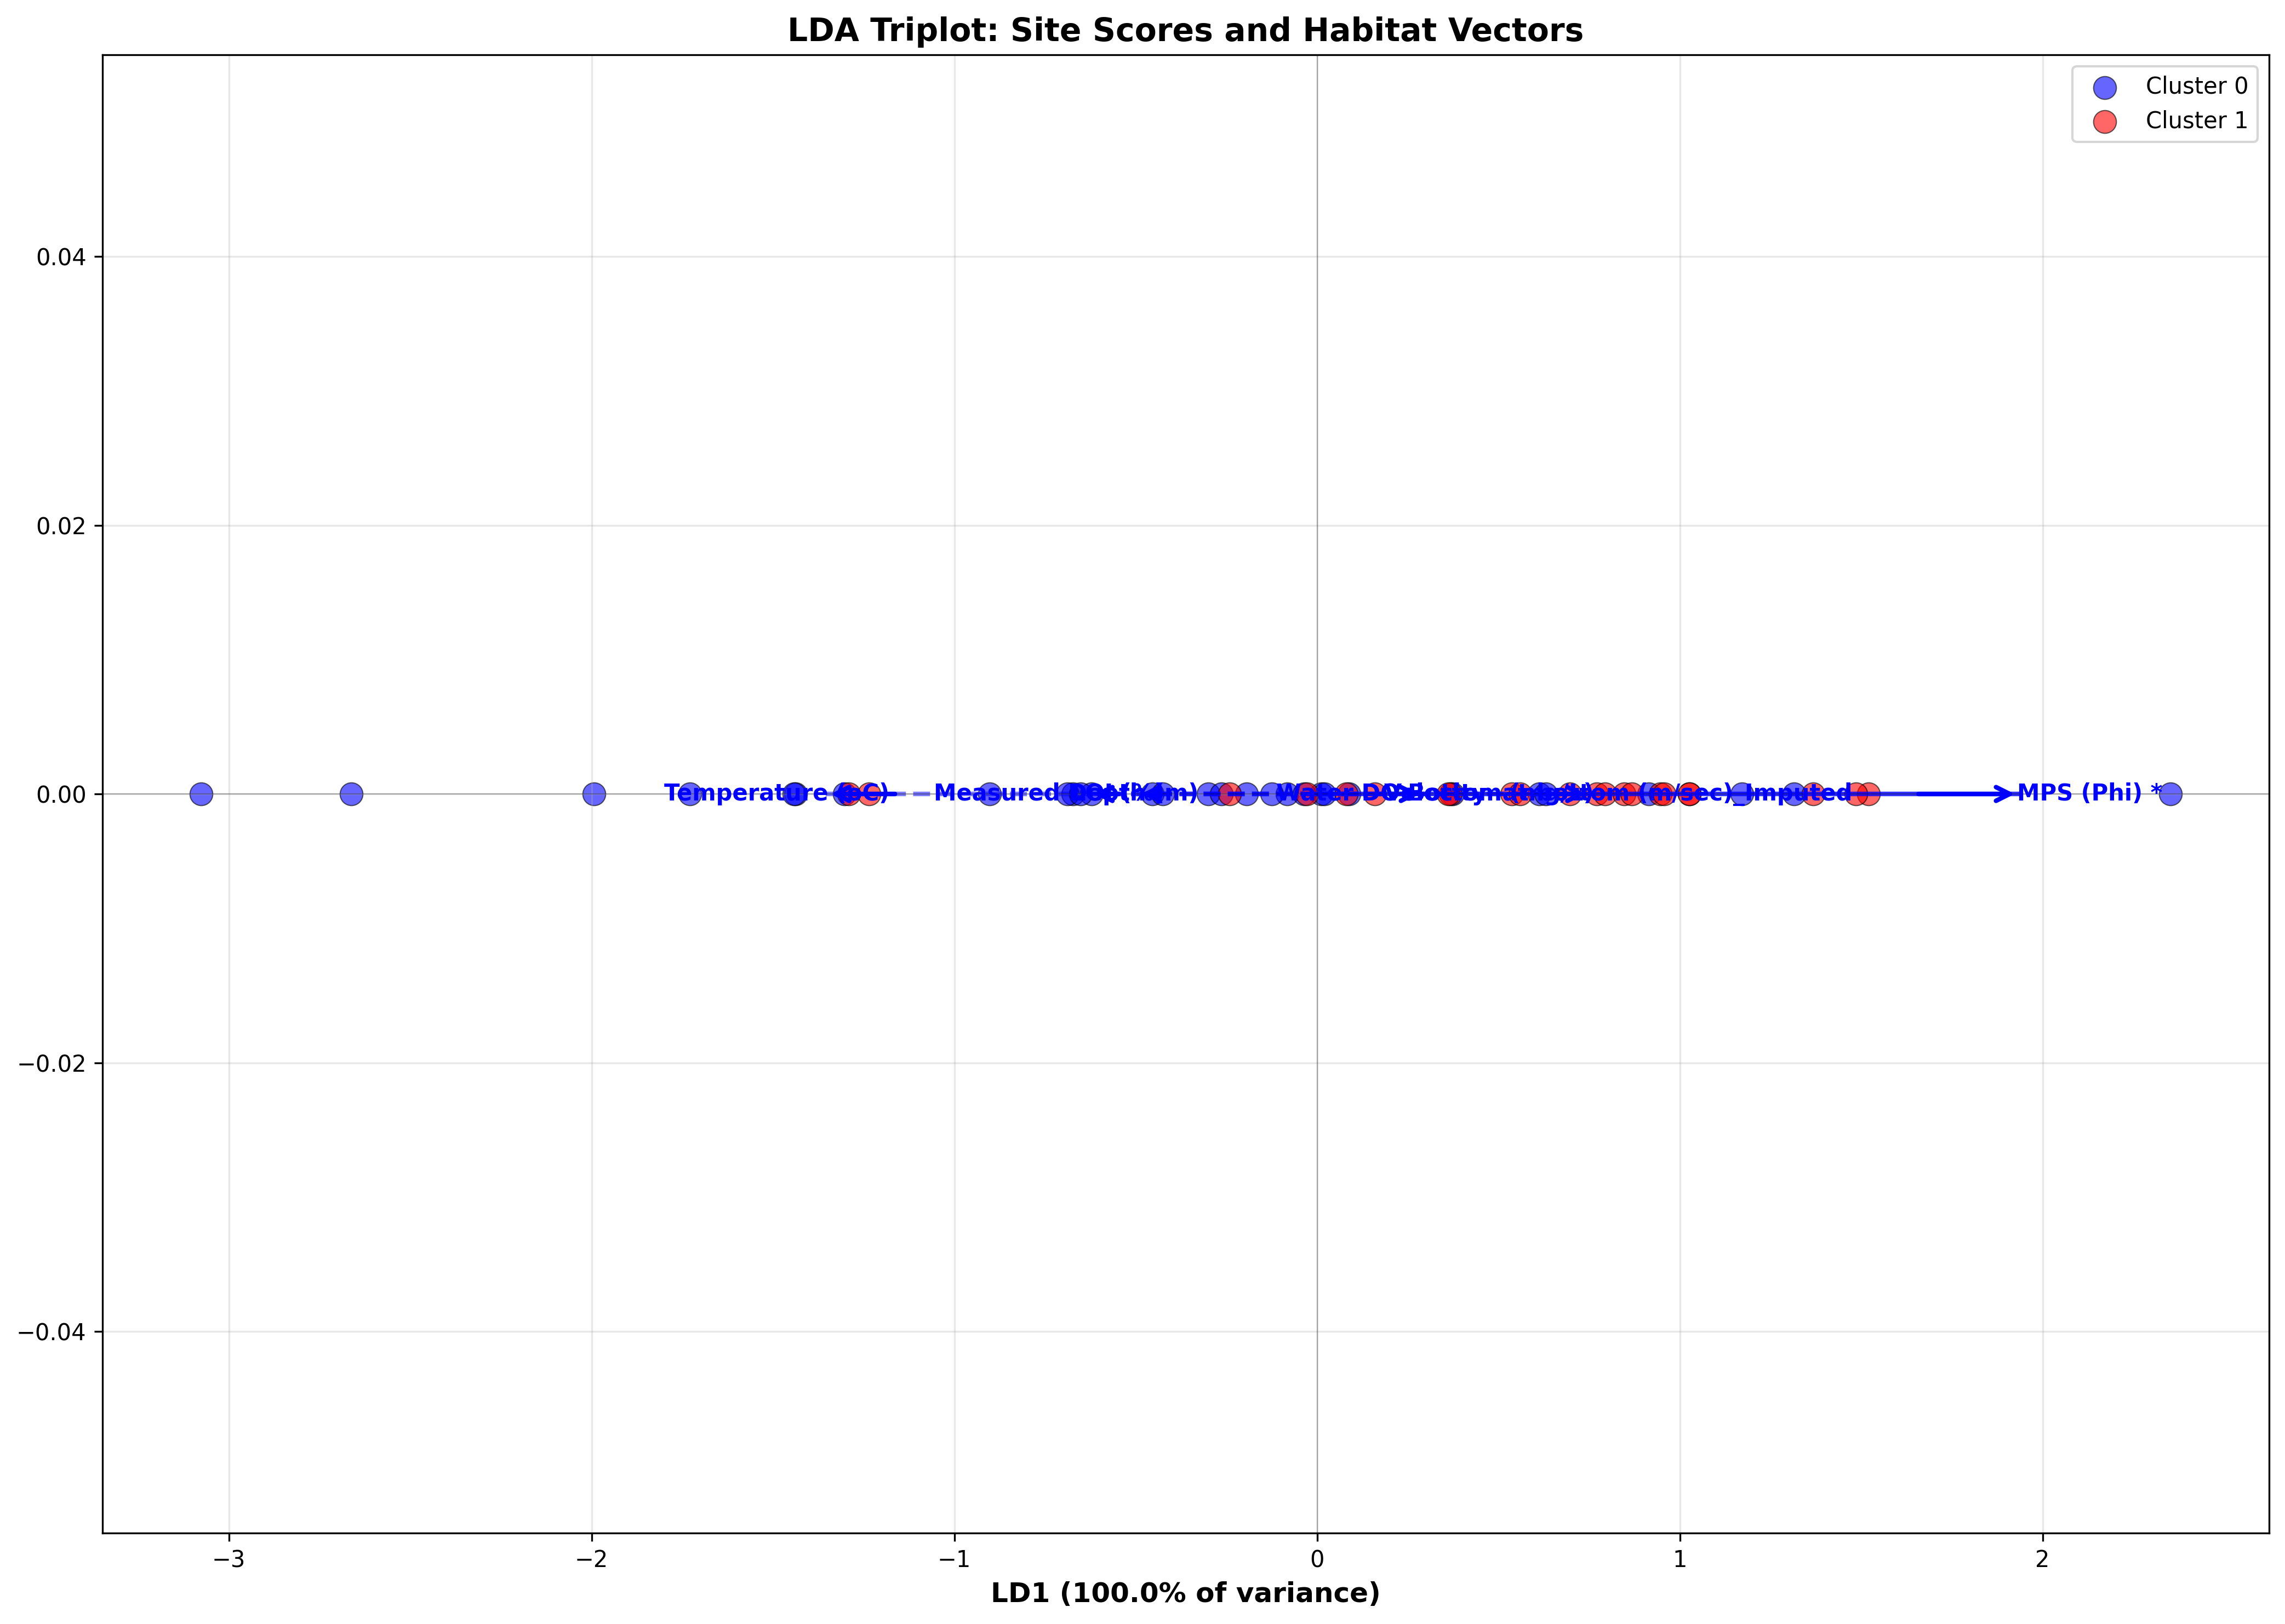
\includegraphics[width=0.9\textwidth]{../results/figures/03_env_driven_taxa_clusters/figure3_lda_triplot.png}
%     \caption{LDA Triplot}
%     \label{fig:03_lda_triplot}
% \end{figure}

\begin{figure}[htbp]
    \centering
    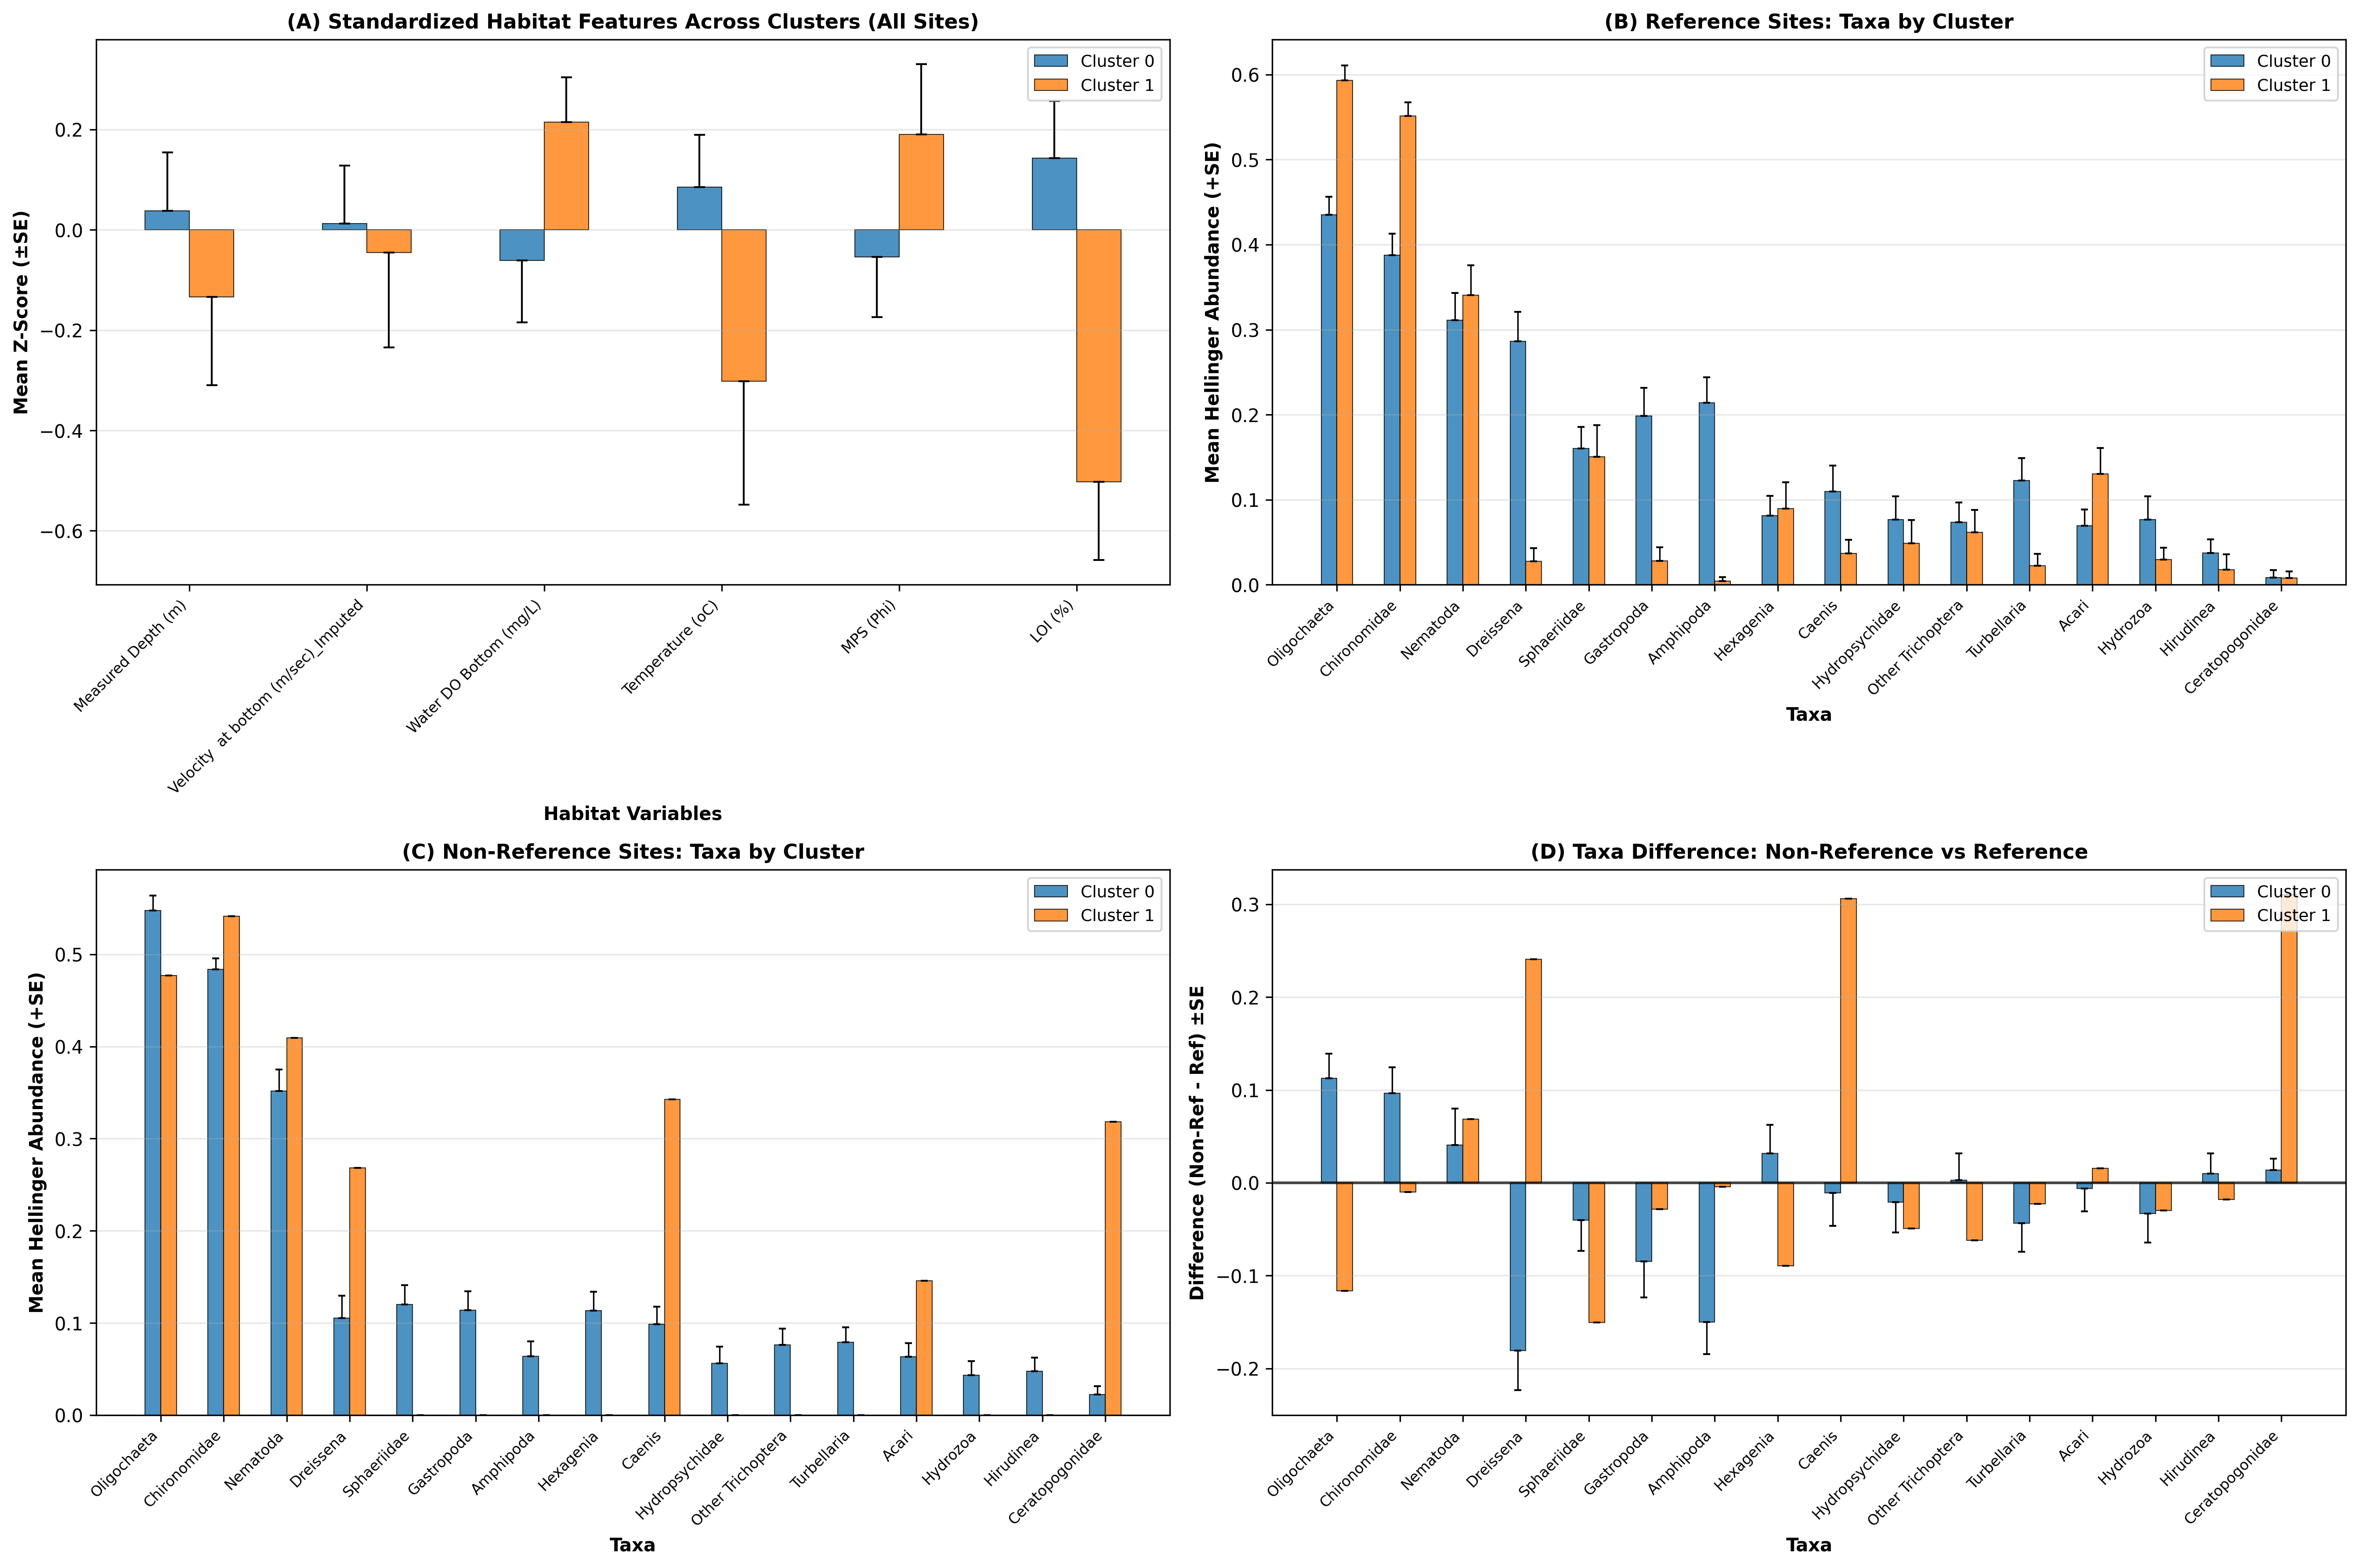
\includegraphics[width=0.9\textwidth]{../results/figures/03_env_driven_taxa_clusters/figure4_cluster_comparison.png}
    \caption{Cluster Comparison}
    \label{fig:03_cluster_comparison}
\end{figure}
